\section{Наибольшая общая абелева подстрока}
\begin{problem}
Даны две строки $a, b \in \Sigma^n$. Нужно найти наидлиннейшую строку $x$ такую, что $xs_a \equiv a, xs_b \equiv b$ для некоторых $s_a, s_b$.
\end{problem}
% Описываешь задачу

\subsection{Общий алгоритм}

Отметим, что нас интересует детерменированный алгоритм решения задачи. Известно несколько недетерменированных решений, на практике работающих достаточно быстро, но они не являются темой исследования данной работы.

Будем подходить к лучшему решению по шагам от самого простого, на каждом шаге оптимизируя какую-то часть алгоритма, для лучшего понимания.

\subsubsection{$(n^2 \log \Sigma, n \log \Sigma)$ w.h.p}

Будем перебирать все длины $l$ и проверять, есть ли общая абелева подстрока длины $l$.
План: построить $P(t)$ для всех $t$ таких, что $|t|=l$, и $a=xty$ для некоторых $x, y \in \Sigma^*$. После этого проверить, есть ли такая строка $r$, что $|r|=l, b=xty, P(r)=P(t)$ для некоторого $t$.

Будем строить векторы $P(t)$ для всех подстрок длины $l$ строк $a$ и $b$ по очереди, переходя от одной подстроки к следующей. Для этого нужно уметь удалять первый символ текущей строки и дописывать в конец новый символ.

Хранить векторы $P(t)$ будем в персистентном массиве, реализованном на персистентном дереве отрезков. Для того, чтобы перейти к следующей строке, нужно уменьшить значение в одной ячейке на 1, и увеличить значение в другой ячейке на 1.

Для того, чтобы научиться сравнивать на равенство две вершины дерева, соответствующие двум векторам $P(t)$, будем при построении считать некоторый хеш от вершины. Будем поддерживать хешмап, в котором для пары хешей $<h_1, h_2>$ хранится хеш от пары этих чисел, если она уже встречалась. Чтобы посчитать хеш для листа, проверим что-нибудь вроде пары $<-pos, val>$ а для внутренней вершины уже точно посчитаны хеши сыновей $<h(v_l), h(v_r)>$. Когда нам нужно узнать хеш пары $<h_1, h_2>$, смотрим в мап: если там есть элемент с таким ключом, достаем оттуда соответствующий хеш, иначе кладем туда новый элемент с таким ключом и значением, равным размеру мапа. Значения всех хешей будет принимать значения от $0$ до $MapSize - 1$.

Таким образом, после подсчета хеша каждой вершины, для всех подстрок длины $l$ первой и второй строки можно выписать их хеши, и нужно проверить, есть ли в двух массивах одинаковое число. Поскольку все значения не превышают $n \log \Sigma$, это можно сделать используя сортировку подсчетом.

Время работы~--- $n$ итераций по $l$, и $n \log \Sigma$ операций для каждой длины: каждая вершина дерева отрезков создается за $O(1)$ w.h.p. используя хешмап. Расходуемая память $n \log \Sigma$ на хранение дерева отрезков и хешмапа.


\subsubsection{$(n^2 \log \Sigma, n^2)$ deterministic}

Посмотрим внимательнее на персистентное дерево отрезков из предыдущего решения. Это ациклический орграф, в котором каждая вершина имеет свой уровень (глубину) от $1$ до $\log \Sigma$, при чем на каждой глубине по $O(n)$ вершин.

Будем считать хеши всех вершин поднимаясь по уровням от листьев к корням, используя один хешмап размера $O(n^2)$, который умеем очищать за $O(1)$.

База: посчитать хеши от листьев. Хеш листа~--- $h(<-pos, val>)$, и $pos$, и $val$ принимают значения порядка $O(n)$. Поэтому можно пройти по всем листам в дереве, и посчитать хеш, обращаясь к хешмапу напрямую и спрашивая, был ли уже такой же лист, и какой у него хеш. Для того, чтобы обойти все листы за их количество, при построении дерева можно в каждый лист складывать ссылку на новый лист, который появляется в следующей версии дерева отрезков.

Переход: посчитан хеш от всех вершин более глубокого уровня. Обратим внимание, что поскольку на каждой глубине $O(n)$ вершин, хеши этих вершин так же будут принимать значения $O(n)$. Поэтому мы можем очистить хешсет и точно так же, как и для листьев, считать новое значение хеша, проверяя, была ли уже такая пара $<h(v_l), h(v_r)>$.

Таким образом, мы построили дерево и посчитали хеши всех вершин за $(n^2 \log \Sigma, n^2)$ полностью детерменированно.


\subsubsection{$(n^2 \log \Sigma, n)$ deterministic}

Начнем с того, что на хранение дерева отрезков у нас сейчас уходит $n \log \Sigma$ памяти, это много. Чтобы уменьшить потребление памяти, можно использовать технику \textbf{limited node copying}. Краткое введение, которое будет необходимо для дальнейшего понимания алгоритма:

Вместо того, чтобы после пересоздания очередного листа пересоздать весь путь до корня, будем хранить в каждой вершине дополнительный указатель, изначально нулевой. Когда мы стоим в вершине и знаем, что один из ее сыновей был изменен, в случае, если дополнительный указатель еще не занят, просто установим его на новую версию этого сына и подпишем текущим глобальным временем. После такого изменения все еще несложно обратиться к какой-то версии дерева отрезков: нужно просто при переходе к сыновьям при выборе, куда спускаться, посмотреть, не нужно ли идти по дополнительному указателю.

Можно доказать, что таким образом построенное дерево занимает $O(n)$ памяти, но не будем об этом.

Подсчет хешей для листьев и внутренних вершин в этом решении отличается.

База: подсчет хешей для листьев. Будем считать хеши листьев группами, для каждой позиции все листья, соответствующие одной позиции в массиве вместе. Будем поддерживать счетчик $ch$~--- первый еще не использованный хеш. Фиксировав, какую позицию мы сейчас обрабатываем, просто обойдем все листья с этой позицией (для этого можно хранить в каждом листе ссылку на предыдущий лист этой позиции), и листу со значением $val$ присвоим хеш $ch+val$, после чего увеличим $ch$ на $max(val)+1$.

Переход: посчитали хеши всех (даже больше, об этом далее) вершин на предыдущем уровне. Кроме хешей для вершины мы записываем не только эту вершину, а еще и все ее копии во все времена, которые мы не создавали явно в дереве отрезков (при переходе на послеследующий уровень их можно безопасно удалить, чтобы сохранить линейную память). Чтобы получить для вершины список всех времен, когда она должна была бы существовать без сжатия, нужно просто взять список всех времен всех трех ее сыновей и смерджить. Пусть у очередной вершины хеши сыновей $h_1$ и $h_2$ (можно считать $h_1 < h_2$). Запишем в вектор с номером $h_1$ напоминание: надо бы посчитать $h(<h_1, h_2>)$ и записать его в текущую вершину $v$. После того, как сделали это для всех вершин текущего уровня, можно идти по $h_1$, очищать хешмап на $O(n)$, и перебирать соответствующее ему $h_2$. Как обычно, если оно есть в хешмапе, достаем оттуда хеш, иначе сопоставляем ему новый. 

После того, как хеши всех вершин посчитаны, можно освобождать память с предыдущего уровня и переходить к следующему. В конце получим посчитанные хеши для всех корней.

Используемое время так и осталось $O(n^2 \log \Sigma)$, а вот требуемая память стала всего $O(n)$.


\subsection{Случай бинарных строк}
% Здесь описываешь алгоритм для бинарных строк
Отдельный интерес представляет случай $|\Sigma|=2$. Есть известный алгоритм, описанный, например, в [1], работающий за время $O(n^2/\log n)$.

В этой же статье рассмотрена задача матожидания длины $LCAF$ двух случайных строк длины $n$ и сделано предположение 5.1 о том, что $LCAF_{avg} \ge n - O(\log n)$. Это преположение выглядит слишком смелым, рассмотрим эту задачу подробнее.

%Для начала рассмотрим график $LCAF_{avg}$ от $n$~--- матожидания длины НОАП в зависимости от длины строк. График получен генерацией $10\,000$ случайных строк соответствующей длины и усреднением результатов.

%\{ График картиночкой \}

%\begin{table}
%\begin{tabular}{|c|c|}
%\hline
%$n$ & $LCAF_{avg}$ \\
%\hline
%1000 & 827.277 \\
%2000 & 1651.76 \\
%3000 & 2487.35 \\
%4000 & 3310.42 \\
%5000 & 4137.15 \\
%6000 & 4960.17 \\
%7000 & 5796.39 \\
%8000 & 6636.79 \\
%9000 & 7452.33 \\
%10000 & 8295.32 \\
%\hline
%\end{tabular}

Этот график никак не похож на $n - O(\log n)$. Более того, можно доказать другое более сильное утверждение:

\begin{theorem}
Для любой функции $f(n)=o(n)$ верно что для двух случайных бинарных строк длины $n$: $LCAF_{avg} < n - f(n)$.
\end{theorem}
\begin{proof}
%От противного. Предположим, что есть функция $f(n)$ и некоторая константа $\alpha<1$ что $LCAF_{avg} >= n - f(n)$, и $f(n) = o(n^\alpha)$.

Лемма: для любой функции $f(n)=o(n)$ с вероятностью $P>0$ верно $LCAF < n - f(n)$.

Обратим внимание, что $f(n) = o(n^\alpha) = o(n)$. Кроме того, центральная подстрока длины $n-2f(n)$, полученная отрезанием суффикса и префикса длины $f(n)$, является подстрокой любой строки длины $n-f(n)$ этой же строки.

Рассмотрим задачу как задачу случайного блуждания: пусть $x_i = A_i - B_i$, где $A, B$~--- наши случайные строки. От стандартной задачи случайного блуждания она отличается тем, что кроме переходов $|x_{i+1}-x_i|=1$ разрешены переходы $x_{i+1}=x_i$. Абелево равенство двух подстрок $A$ и $B$ эквивалентно тому, что подпуть блуждания $x$ возвращается в свое начало, $x_r=x_l$.

Наше случайное блуждание имеет следующие вероятности:

\begin{tabular}{|c|c|}
\hline
$\Delta x$ & $p(\Delta x)$ \\
\hline
-1 & 0.25 \\
\hline
0 & 0.5 \\
\hline
1 & 0.25 \\
\hline
\end{tabular}

$P(n, k)$~--- вероятность после $n$ испытаний получить сумму $k$. Можно заметить, что $P(n, k)=C(2n, n+k)\cdot 2^{-2n}$. И действительно, если посмотреть на геометрический смысл этого распределения, то $P(n,k)$~--- вероятность за $2n$ равновероятных шагов вправо или вверх дойти до диагонали $x+y=2n$ и остановиться на диагонали $y-x=k$, что сходится с формулой $P(n,k)=P(n-1,k-1)+2P(n-1,k)+2P(n-1,k+1)$.

При больших $n$ будем приближать наше биномиальное распределение нормальным, $P(n, k)=\sqrt n N(0,1)$ %(WARNING, CHECK CONSTANT)

По закону трех сигм можно сказать, что у центрального пути длины $n-2f(n)$ вероятность остановиться в промежутке $[-3\sqrt{n-2f(n)}; 3\sqrt{n-2f(n)}]$ около 0.9973, а поскольку $f(n)=o(n)$, вероятность того, что изменение координаты окажется вне промежутка $[-3\sqrt{n}; 3\sqrt{n}]$, хотя бы 0.0026. %(WARNING, считаю, что f(n)=o(n) ---> \_очевидно\_, что можно выкинуть f(n) оттуда)

Для того, чтобы получить отрезок длины $n-f(n)$ с нулевой суммой, нужно взять какой-то суффикс префикса длины $f(n)$ и какой-то префикс суффикса длины $f(n)$. Покажем, что с достаточной вероятностью мы не сможем приблизиться к нулю за $f(n)$ шагов:

Скажем, что наше блуждание сейчас будет обычным случайным, с двумя переходами +1 и -1. Этот переход лишь делает оценку строже, т.к. можно продлить все испытания, в которых был переход по 0 до ровно $k$ ненулевых переходов и прийти к случайному блужданию, при чем максимум модуля отклонения на префиксе мог только увеличиться.

Есть известный факт, что в случайном блуждании если мы находимся в 0, и заканчиваем, когда попадем в точку с координатой $a$ или $-b$ ($0 < a, b$), то матожидание шагов до этого события $ab$. Воспользуемся этим: матожидание количества шагов до момента, когда мы попадем первый раз в точку $-\sqrt n$ или $\sqrt n$, равно $(\sqrt n)^2=n$. Поскольку матожидание равно $n$, значит существует вероятность $C>0$, с которой весь наш путь из $n$ шагов будет в полосе $(-\sqrt n, \sqrt n)$. %(WARNING, доказательство не оч из-за $C$, надо поаккуратнее)

Таким образом, с вероятностью хотя бы 0.0026 центральный подпуть будет иметь отклонение от нуля хотя бы в $3\sqrt n$, и с вероятностью хотя бы $C^2$ и префикс, и суффикс, который мы допишем к этой строке, будут иметь отклонение не больше, чем на $\sqrt n$, то есть, с вероятностью $P>=0.026C^2$ у двух случайных строк наибольшая абелева подстрока будет меньше, чем $n-f(n)$.

Вернемся к доказательству теоремы. Будем доказывать ее от противного~--- пусть есть $f(n)=o(n)$ такое, что $LCAF_{avg} >= n - f(n)$. 

Оценим $LCAF_{avg}$. По лемме, с вероятностью $P>0$ $LCAF$ будет не больше, чем $g(n)=\sqrt{nf(n)}$. Тогда

$LCAF_{avg} <= P (n-g(n)) + (1-P)n = n-Pg(n) < n - f(n)$, т.к. $f=o(g)$. Противоречие.

\end{proof}

Кроме того, докажем грубую оценку снизу:
\begin{theorem}
Для двух случайных бинарных строк длины $n$: $LCAF_{avg} \ge 0.05n$.
\end{theorem}
\begin{proof}
Снова приблизим наше случайное блуждание нормальным распределением и воспользуемся правилом трех сигм.
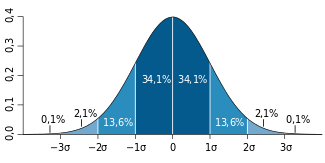
\includegraphics[scale=1]{pics/3sigm.png}

С вероятностью $2 \cdot 0.34$ за первые $n/2$ шагов мы остановимся в зоне $[-\sigma; \sigma]$. После этого, с вероятностью хотя бы $0.136+0.021+0.001 \ge 0.15$ мы за следующие $n/2$ шагов пройдем в другую сторону хотя бы $\sigma$ шагов, обязательно перейдя через точку старта. Таким образом, с вероятностью хотя бы $2 \cdot 0.34 \cdot 0.15$ НОАП будет хотя бы $n/2$, или $LCAF_{avg} \ge 0.05$.

\end{proof}

%\end{table}